\chapter{Analysis of an interesting AME region: $\lambda$~Orionis}

 \section{An interesting AME region}
		The $\lambda$~Orionis molecular ring \footnote{Also known as the Meissa Ring} is a massive stucture surrounding the $\lambda$~Orionis O-type star. The ring contains an HII region, ionized by LOri itself and its OB associates \citep{murdin77}. What had been thought of as a star\-forming region of missing molecular gas
    \footnote{At the time \cite{murdin77} even speculated that this could be evidence of an alternate star\-formation pathway, writing: ``Notably we need to know if $\lambda$Ori is an example of a different mode of star formation or [...] simply a case in which the progenitor molecular cloud was exhausted within the last one or two million years.''}

    \cite{maddalena86,maddalena87}.  (and references therein) noted a ring of material likely being pushed out by the central, historically well-known Lambda Orionis Association of B-type stars and surrounding HII reigon.

   \subsection{Where does the ring come from?}
    \cite{cunha96} argued that the ring may have resulted from a supernova explosion, further speculating that LOri may have been a companion of the progenitor
    \footnote{LOri is a known binary system, with its current companion being a B-type star. \citep{murdin77}}
  .
     The central region is heated by the $\lambda$Orionis star itself, and the Orion~OB association it belongs to \citep{ochsendorf15}. The region is known to host several young stellar and protostellar objects \citep{koenig15}.

    At approx. 10$^{\circ}$ wide, we can see the outline of the structure even in the low (1$^{\circ}$ FWHM) resolution PCAME map. The ring shape itself is thought to originate from a supernova, or perhaps combined effects of the entire star formation history of the Lambda Orionis Association, including the formation of its surrounding HII region \citep{aran09}.

  \subsection{A well-studied region}
    Although the LOri region has been a popular target for study since approximately 1982 \footnote{\cite{duerr82} wrote of the relative lack of work on the overall region: ``Surprisingly, this interesting complex has been little studied''}, fewer works had looked into the ISM structure of the entire region.  Many works have investigated the astrophysics of individul portions of this region. The large angular size is such that all-sky surveys were a natural boon for study of such extended structures. WISE especially was a huge source of insight \citep{koenig15}. More recently, the region was strongly highlighted by a Planck Collaboration microwave foregrounds follow-up investigation, as a strong candidate for further AME investigation \citep{planck15XXV}.


	\section{Investigative approach}

      We have carried out an initial comparison of the AME of this region with its mid to far-IR dust emission. The region is shown in Fig. \ref{fig:orionis-akari9} as it appears in 1$^{\circ}$-smoothed A9 data\footnote{Images at each wavelength used here are included as in appendix to this thesis}. The ring structure itself indicates excess microwave emission attributed to AME (white contours) while the central region is dominated by free-free emission \citep{aran09, koenig15,planck15XXV}. Taking the hint from \cite{planck15XXV} that this may be among the more reliably component separated regions appearing in the PCAME map, we evaluate if there is any preferential relationship between any parameter of dust emission and the AME.

		\subsection{Data preparation}
			As indicated in Ch. \hyperref[ch:datasources]{\ref{ch:datasources}}, we use 12 photometric all-sky maps. For the IRC data (A9 and A18), we produce mosiacs of LOri from the individual tiles provided in the internal all-sky archive.\footnote{IRC all-sky data is still in the proprietary phase at the time of this writing, but should be public by April 2018.} For the other sources, HEALPix all-sky maps are available publicly, at sufficient resolution relative to their native resolutions. \footnote{Planck data was retreived from the NASA IPAC online archive at \url{http://irsa.ipac.caltech.edu/data/Planck/release_2/all-sky-maps/}}\footnote{AKARI/FIS data }\footnote{IRAS/IRIS data }

		\subsection{Extraction from HEALPix maps}
		  For the data obtained via HEALPix maps, we employ the ``healpix2wcs'' functionality provided in the ``gnomdrizz'' python package\footnote{Available at \url{http://cade.irap.omp.eu/dokuwiki/doku.php?id=software}}\footnote{``drizzlib'' 1.2.2 and earlier were not able to correctly access HEALPix files with multiple fields/columns. See appendix for our recommended workaround.} A9 and A18 images are produced by regridding the images with the ``montage'' software by NASA/IPAC. All of the images for all of the bands are based on a common FITS header which has a pixel grid spacing equal to the average pixel width in the NSIDE 256 HEALPix scheme.
      A background estimation and subtraction is made

		\subsection{Multi-wavelength characterization}
			Figure \ref{fig:orionis-img} shows the region in 12 photometric bands, from the mid to far IR. Contours indicate the region's shape in the PCAME map. Figure \ref{fig:orionis-corr} shows IR to AME cross correlation plots, for all pixels within the 10$^{\circ}$ by 10$^{\circ}$ $\lambda$~Orionis region. The correlation is most clear for the shortest and for the longest wavelength bands, and weakens the most at around 60~$\mu$m. The weakening of the correlation score appears to come from brighter 25 to 90~$\mu$m emission within the ring. The spectrum is consistent with warm thermal dust emission, heated by $\lambda$~Orionis and its associates. The ring structure itself appears relatively consistent accross all bands. Fig. \

		\subsection{Ionization fraction}
			We attempt to estimate the relative fraction of charged to neutral PAHs via the R(A9:I12) band ratio. A9 is known to cover ionized PAH features (as well as neutral) whereas I12 primarily covers neutral features.
      %Fig. \ref{fig:lori_RA9I12} indicates that R(A9:I12) correlates with $AME_{var}$


\begin{figure*}
  \label{fig:orionis-akari9}
  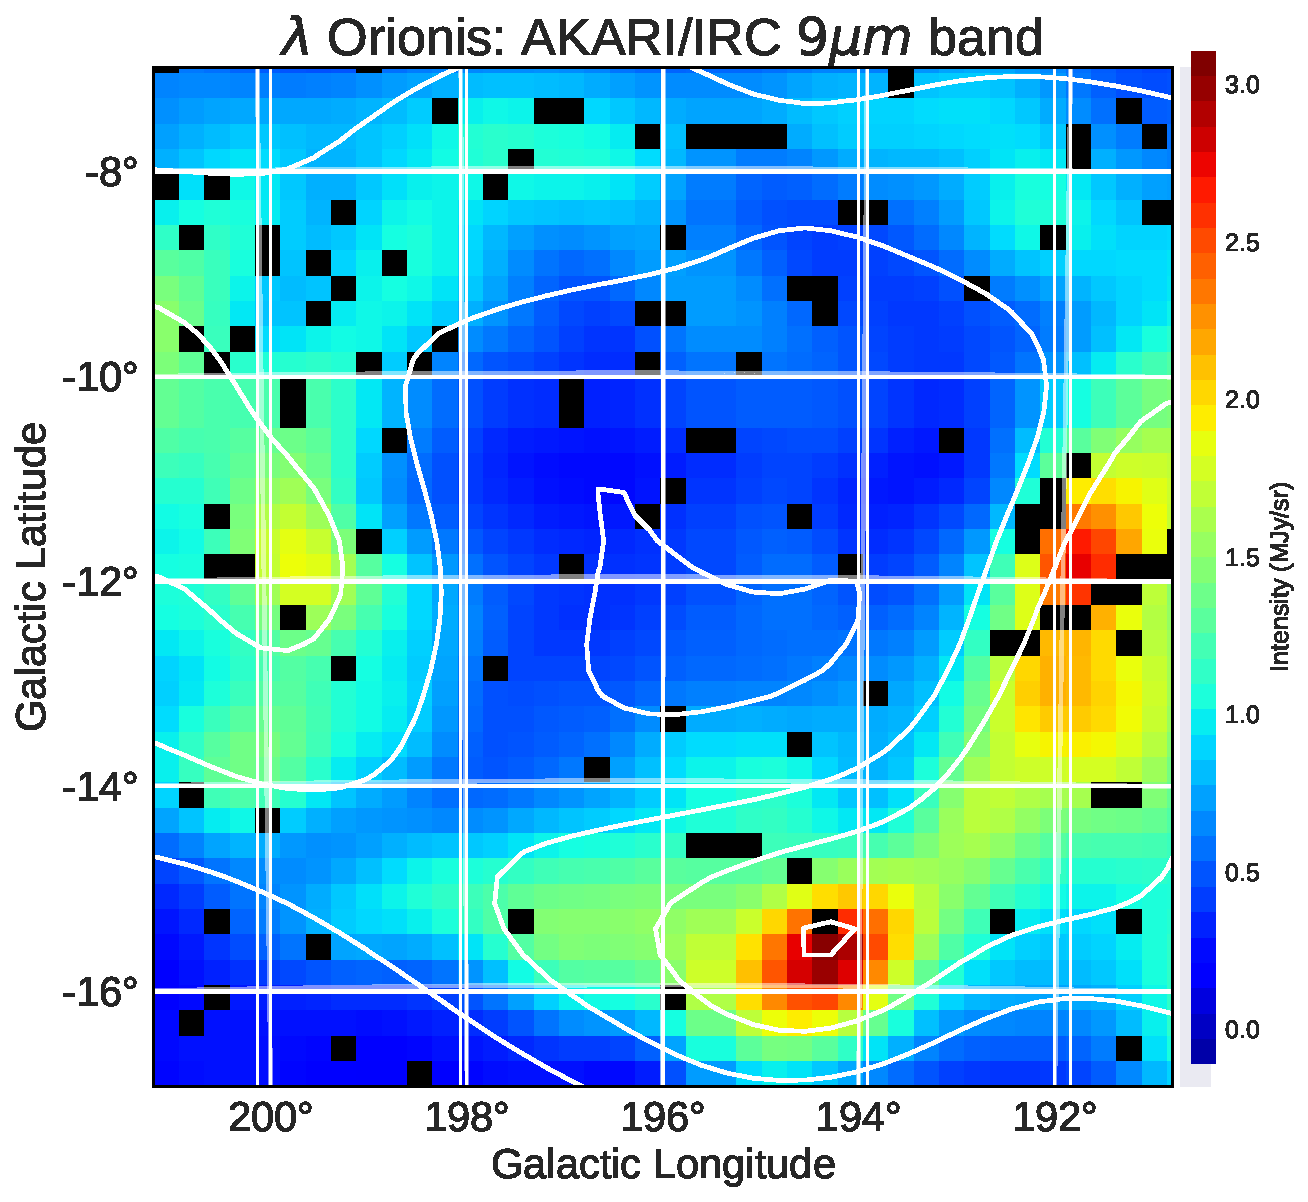
\includegraphics[width=\textwidth]{../Plots/LOri_akari9_AMEcont_1dres.pdf}
  \centering
  \caption{$\lambda$~Orionis as it appears in the AKARI 9~$\mu$m data. Contours indicate the AME, as given by the Planck PR2 AME map. The image is smoothed to a 1$^{\circ}$ PSF (much larger than the original 10 arcsec map. The $\lambda$~Orionis star itself is approximately located at the center of the image.
  %The dust wave structure, described by *citation needed*, is apparent, and seems to coincide with a local maxima in the PR2 AME contours. The units are MJy/sr. )
  }
\end{figure*}

\begin{figure*}
  \label{fig:orionis-img}
  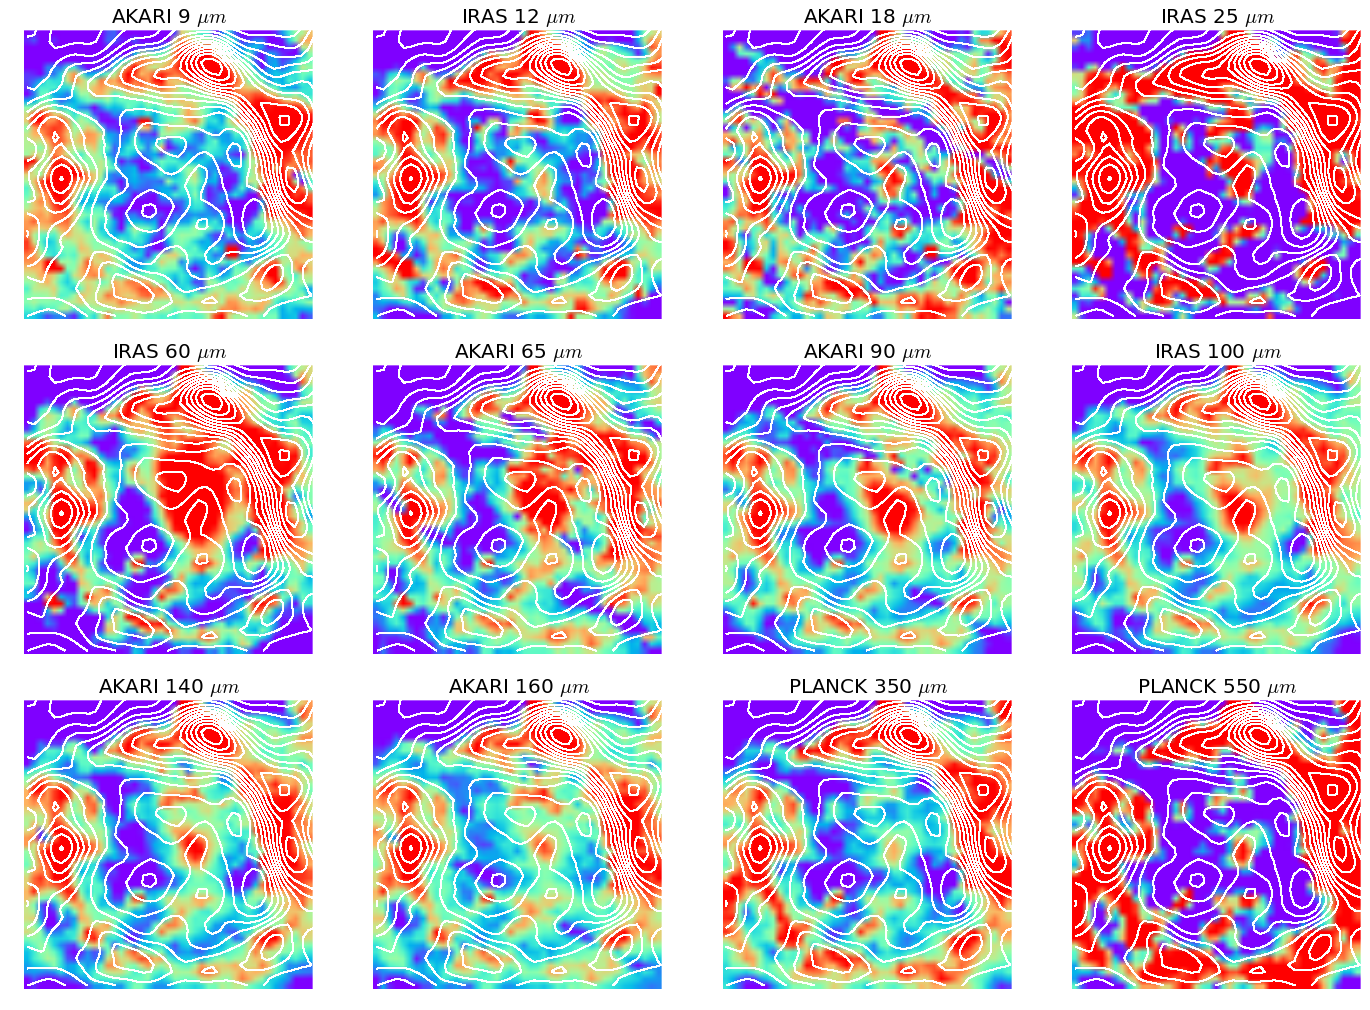
\includegraphics[width=\textwidth]{../Plots/lOrionis_grid_img.png}
  \centering
  \caption{A grid of thumbnails showing the $\lambda$~Orionis region's structure, at 12 wavelengths, along with AME contours (shown in white countours. Spatial correlation seems to be the best at the shortest and longest wavelengths (AKARI/IRC 9~$\mu$m and Planck/HFI 550~$\mu$m). The images are smoothed and interpolated for demonstration. Figure \ref{fig:orionis-akari9} demonstrates the actual pixel grid used for the SED fitting and intensity correlation tests.}
\end{figure*}

\begin{figure*}
  \label{fig:orionis-corr}
  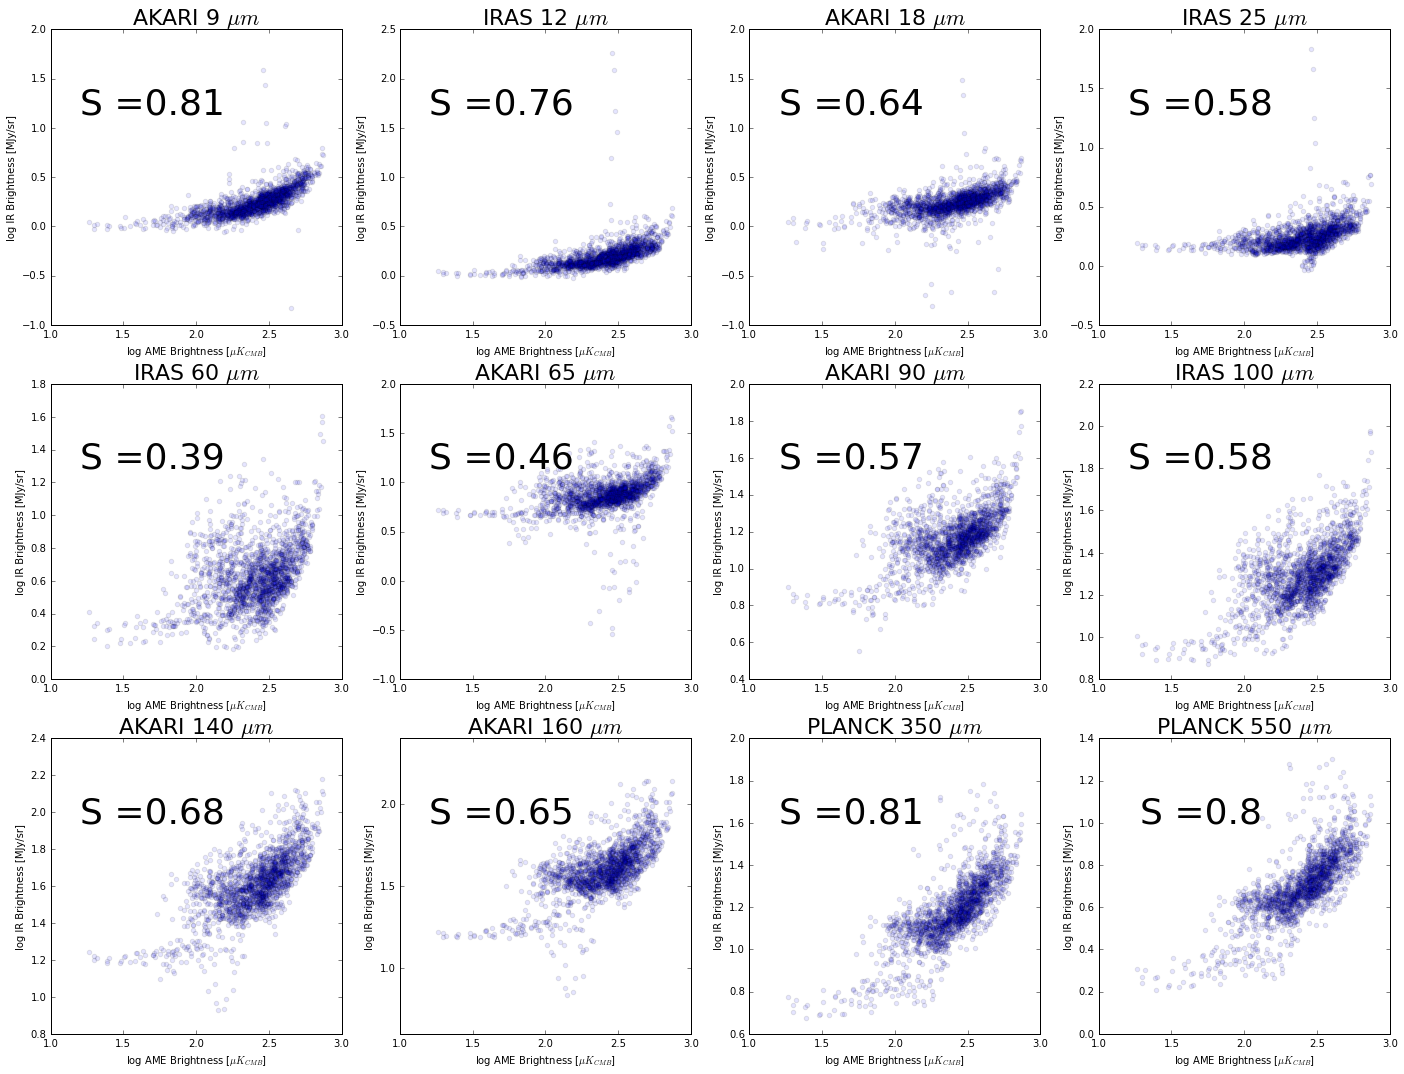
\includegraphics[width=\textwidth]{../Plots/orionis_correlations_AME.png}
  \centering
  \caption{Pixel cross-correlation for all pixels in the $\lambda$~Orionis cut-out region.  $r_{s}$ indicates the Spearman rank correlation coefficient for each plot.}
\end{figure*}

\subsection{SED Fitting}

We performed a full dust SED fitting on the LOri photometry, according to the \cite{galliano11} dust model. We used a mixture of amorphous carbon and silicate dust. Indeed, this dust mixture is more emissive than the standard silicate-graphite \citep{draine07}, by a factor of 2-3. As was shown by Herschel, in the LMC \citep{galliano11}, and by Planck, in the Milky Way \citep{planck16}, this increase of emissivity is necessary to have a proper fit of the sub-mm emission. We assume that the radiation field heating this dust mixture is the Galactic ISRF \citep{math83}, scaled by a factor $U$. We also assume, following \cite{dale01}, that the dust is exposed to a distribution of starlight intensity, distributed as:

\begin{equation}
   \label{eq:U}
     dM_{dust}\propto{} U^{-\alpha}dU
\end{equation}

between $U_{min}$ and $U_{max}$, where $U_{min}$, $U_{max}$ and $\alpha{}$ are free parameters. An old stellar population template (PEGASE; \citep{fioc97}) is added to this SED in order to model the near-IR emission. We perform a simple least-squares analysis.
